\section{Sealed Evaluation: Accuracy and Alarm Cost}
\label{sec:c01-results}

The five-model bank makes \COneMixTimely{}/\COneMixTotal{} timely
family-and-source decisions with \COneMixExtras{} unmatched event-stream
alarms. Its nominal counterpart makes \COneNomTimely{}/\COneNomTotal{}
with \COneNomExtras{} extras. The frozen causal ExtraTrees reference makes
\COneETTimely{}/\COneETTotal{} with \COneETExtras{}; its short-window
variant makes \ReaderETShortTimely{}/\COneETTotal{}
with \ReaderETShortExtras{} extras. These are paired
replays of 108 interventions, not 648 independent events. Figure~\ref{fig:c01-main}
shows why the totals differ: the physical banks recover nearly all loads,
while both learned adapters already recover most tested lines. The extra
alarm burden of the physical banks rises sharply when true R/X changes
fall outside their five-model bank.

\begin{table}[t]\centering\small
\caption{Sealed continuous-stream decisions. Each family has 324 replayed
instances from 108 distinct interventions; extras are unmatched alarms on
event records. The methods retain unequal alarm operating points.}
\label{tab:c01-direct}
\begin{tabular}{@{}lrrr@{}}\toprule
Method & Load & Line & Extras\\\midrule
Physical bank & \ReaderPhysicalLoad/324 & \ReaderPhysicalLine/324 & \COneMixExtras\\
Nominal bank & \ReaderNominalLoad/324 & \ReaderNominalLine/324 & \COneNomExtras\\
ExtraTrees & \ReaderETLoad/324 & \ReaderETLine/324 & \COneETExtras\\
ExtraTrees short & \ReaderETShortLoad/324 & \ReaderETShortLine/324 & \ReaderETShortExtras\\\bottomrule
\end{tabular}\end{table}

\begin{figure*}[t]\centering
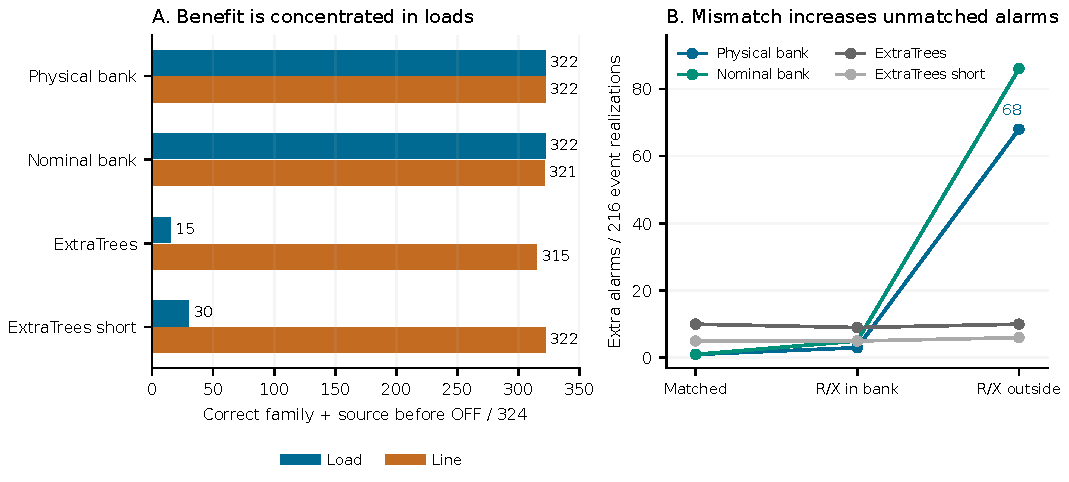
\includegraphics[width=.91\textwidth]{figures/generated/reader_c01_tradeoff.pdf}
\caption{Sealed continuous evaluation. (A) Timely correct family and source
by event family, with 324 paired realizations per family. (B) Unmatched
event-stream alarms across the two noise levels within each R/X condition,
with 216 event realizations per condition. The plots display the gain in load
attribution and the alarm cost under out-of-bank network error together.
Each method retains its own frozen publication rule and false-alarm budget.}
\label{fig:c01-main}\end{figure*}

The paired intervals in Fig.~\ref{fig:c01-ci} confirm a timely-attribution
advantage over this ExtraTrees reference in each tested stratum. They also
show a higher rate of unmatched alarms under out-of-bank R/X. Those
intervals resample physical parents, preserving correlation across noise
replays and network conditions. They do not establish
superiority at a common false-alarm operating point. The physical bank's
stratum median diagnosis delay is about 0.27\,s in matched and in-bank
conditions; the ExtraTrees medians range from 0.19 to 0.30\,s. There is
no general latency advantage.

\begin{figure*}[t]\centering
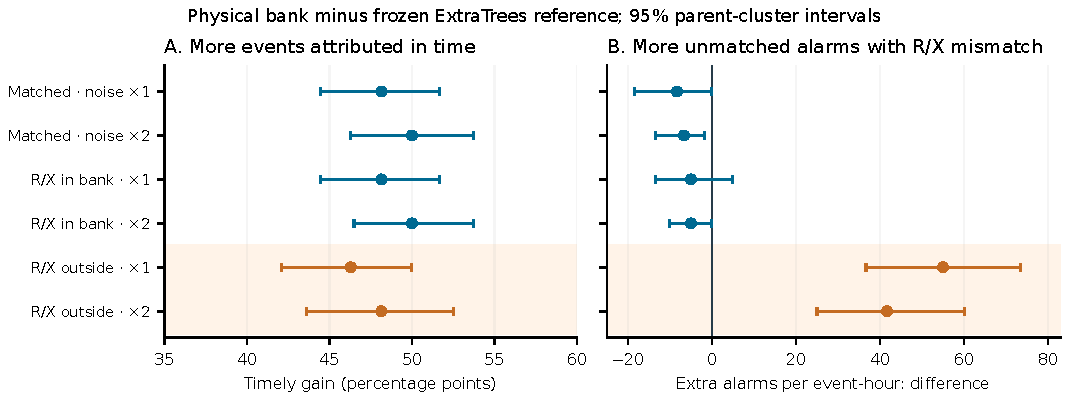
\includegraphics[width=.89\textwidth]{figures/generated/reader_c01_intervals.pdf}
\caption{Physical bank minus frozen ExtraTrees reference in the six paired
strata. Points and 95\% intervals come from 10,000 physical-parent
resamples. Left: percentage-point difference in timely attribution; right:
difference in unmatched alarms per event-record hour, whose denominator
includes the 12-s startup. The orange rows expose the out-of-bank R/X
failure. The intervals describe this finite simulated population.}
\label{fig:c01-ci}\end{figure*}

The separate persistent-line test scores the first stop. Both physical
banks and both ExtraTrees adapters identify the right line first on
162/162 openings. The declared Chen2016 adapter does so on 74/162;
66 records stop before the opening and 22 stop afterward on a wrong line.
It also stops on all 72 paired normal records, whereas the continuous
methods alarm on none. Chen's normal exposure ends at its first stop
(2,522\,s); the other methods monitor 42,336\,s each. These unequal
exposures and the adapter's white-injection assumption prevent a general
claim against published quickest-change detection. Full stratified tables,
failure ledgers, restoration outcomes and censoring are in the supplement.

The experiment establishes performance on the specified nine-load,
nine-line simulator catalog. It does not establish a new hackathon score,
unseen-source generalization, calibrated event probabilities, field
operation or real-time throughput.
